Специфика эксперимента такова, что при заданном сдвиге по звёздной величине (или, что тоже самое, при заданном отношении усилений изображений) неопределённость во временной задержке, вызванная микролинзированием, не зависит от $\Delta t_{\textrm{ист.}}$. В действительности, в реально наблюдаемых изображениях гравитационно линзированных объектов нельзя точно указать отношение усилений, что нельзя не учитывать при более точных исследованиях. Для иллюстрации выбраны следующие значения: $$\Delta t_{\textrm{ист.}}=40, \ \Delta m = -0.28.$$
Для контроля точности временных интервалов между точками вводится сетка с $n$ делениями, так что расстояние вдоль горизонтальной оси между точками составляет $\frac{400}{n}$ дней.

\begin{figure}[H]
    \centering
	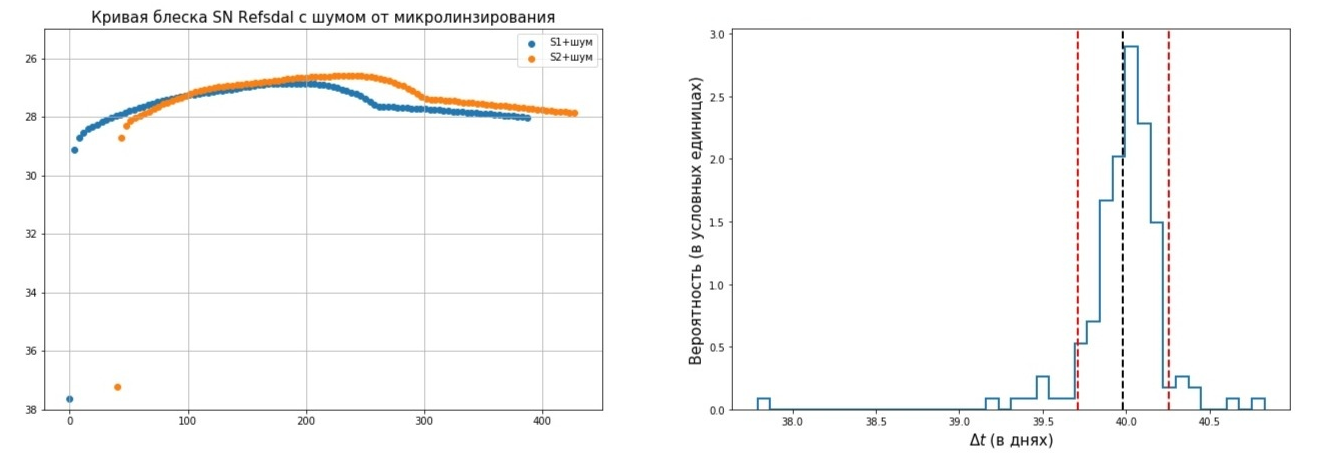
\includegraphics[scale=0.5]{pics/fig10.png}
	\caption{Слева: кривые блеска в изображениях S1, S2 SN Refsdal с шумами от микролинзирования. Справа: гистограмма временных задержек... ПОПРАВИТЬ! \label{fig:proba}} 
\end{figure}